\chapter{Intent Change Estimation Based on Physical Interactions of an	Exoskeleton User}\label{chapter:BKF}
The IMM estimation framework presented previously is reactive as it monitors signs of gait transition i.e.~if the CoM trajectory after gait transition does not resemble library gaits, the IMM algorithm will misidentify the intended change until after it has been realized. However, anticipative intent inference is more desirable to time the assistance delivery appropriately and help the user realize their intended gait transition. Improper assistance timing may result in the robot resisting the user's actions, hampering HRI fluency. Intent may be anticipatively inferred by identifying the actions the user takes to realize their intent change and using data from gait features to detect them. Actions indicative of intent change may be detected by monitoring the interactions the user has with the exoskeleton and the environment. These interactions may provide an earlier indicator of intent changes compared to CoM or joint motions making it possible to anticipate user intent and provide assistance to the user to help realize the desired objective.

\section{Quantifying intent - Enabling estimation}
User intent is an abstract content, so it must be quantified and inferred using a measurable quantity, and this quantification is a design choice. The intended gait speed was chosen to represent user intent as the primary objective of the exoskeletons herein is gait rehabiliation. The state of the exoskeleton user is represented in a vector $ \x = [\mathbf{p}_{CoM}^{\top} ,\mathbf{v}_{CoM}^{\top}]^{\top} $. To capture intent, the state was extended to include the intended gait velocity $ z $ as a hidden state in an augmented state vector $ \q = [\x^{\top} ,z]^{\top} $. This state augmentation approach allows using the Kalman filter to directly estimate the intended gait speed. 

Previously performed studies of bipedal locomotion give us an idea of how changes in walking gaits corresponding to transitions in user intent. These physical indicators include differences in CoM trajectories and foot placement, as illustrated in Fig.~\ref{fig:main_idea}. Ground contacts greatly influence the stability of legged locomotion, so it was hypothesized that intent will be reflected strongly in the user's choice of ground contacts through foot placement \cite{bhounsule2014foot}. Modulating foot placement while walking is an effective control mechanism to maintain stability \cite{hof2010balance,bhounsule2015control}, and it has been shown that velocity changes at MS influence foot placement at TD \cite{wang2014stepping,redfern1994model}. 

\begin{figure}
	\centering
	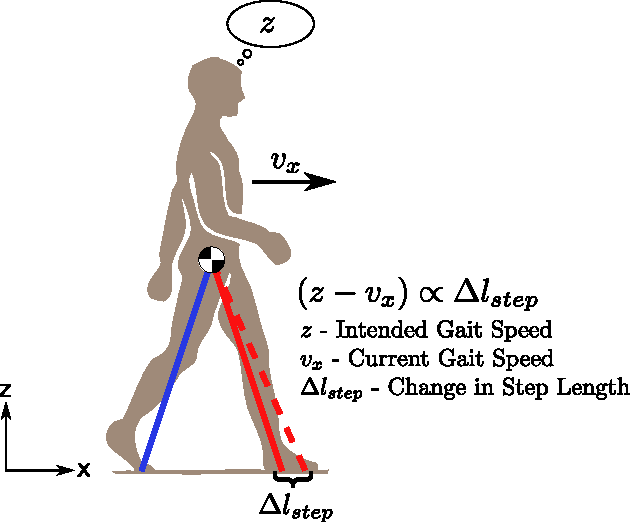
\includegraphics[width=0.5\linewidth]{main_idea}
	\caption{Change in intended velocity may be inferred from change in step length}\label{fig:main_idea}
\end{figure}

The B-SLIP model may be used to adequately model steady-state walking, and foot placement was found to be critical in optimizing periodic gaits. The model does not inherently capture the active changes required to change speed nor the first-principles humans employ for foot-placement as a function of the desired gait speed. These aspects were initially modeled by designing a controller for the B-SLIP model to emulate human motor control. With such a design, intent changes may be considered analogous to controller setpoint changes. Several theories try to explain human motor control, one of which says that the human sensorimotor system relies on optimal control \cite{todorov2004optimality,sylla2014assessing}. Therefore, we chose to assume the human motor controller to be a Linear Quadratic Regulator (LQR). The MS-to-MS Poincar\'e map was linearized about a periodic gait and the linearized model was used to design a controller that minimized deviations from a specified gait. 

The dynamics of the B-SLIP model are nonlinear and linearizing them about a single periodic gait results in a model valid for a very small portion of the gait which rendered the controller unable to handle large speed changes. A derivative-free technique i.e., the Unscented Transform \cite{manchester2016derivative} were employed to generate a linear model. This technique required integrating dynamics backward in time which was difficult to do for the hybrid dynamics of the B-SLIP model as the gait event timing cannot be fixed. Therefore, due to the lack of first principles that describe human choices to bring about intended gait changes, a data-driven approach was chosen to model the relationship between intended gait speed and foot placement.

\begin{figure}
	\centering
	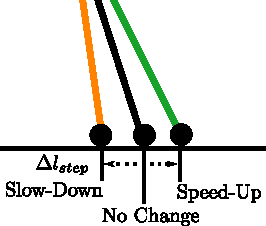
\includegraphics[width=0.4\linewidth]{step_change.pdf}
	\caption{Speed-up and slow-own increase and decrease the step length respectively}\label{fig:step_change}
\end{figure}

It was assumed that intent changes made at MS are reflected in the placement on the foot at TD and then maintained as constant until the following MS. There is a correlation between step length and walking velocity that can be exploited to infer changes in intended gait speed. People walking at lower velocities exhibit shorter step lengths, and an increase in velocity results in an increase in step length \cite{kuo2001simple,andriacchi1977walking}, as illustrated in Fig.~\ref{fig:step_change}. A twice-per-step estimation strategy was considered to make use of the footstep information obtained at TD. As illustrated in Fig.~\ref{fig:step_stages}, the first state update is made at TD when the footstep is finalized and a second at MS.